% SC2000 — Chapter 1: Counting & Combinatorics (0->100 ground-up)
\chapter{Counting \& Combinatorics}
\label{ch:counting}

\begin{quote}
\emph{``Counting is the oldest branch of computing.''} Before probability, before statistics, before machine learning: how many ways can it happen? Every algorithm that enumerates, every cryptographic key space, every dataset split begins with counting.
\end{quote}

\noindent\fbox{\parbox{\dimexpr\linewidth-2\fboxsep-2\fboxrule}{%
\textbf{From zero: no prior combinatorics assumed.} We build from ``how many?'' with pictures before formulas. If you can count on your fingers, you can follow this chapter. Every rule is motivated by a concrete computing scenario.}}
\vspace{0.4em}

\section*{Learning Outcomes}
After this chapter you will be able to:
\begin{enumerate}[label=(L\arabic*)]
    \item apply the multiplication (product) and addition (sum) rules to count compound choices;
    \item count permutations and combinations with and without repetition;
    \item use stars-and-bars, the binomial theorem, and inclusion--exclusion;
    \item apply the pigeonhole principle to prove existence claims;
    \item estimate key-space sizes and algorithmic branching factors.
\end{enumerate}

% ============================================================
\section{Why Counting Matters in Computing}
\label{sec:why-counting}
How many $8$-character passwords over $62$ symbols ($a$--$z$, $A$--$Z$, $0$--$9$)? How many ways to choose $5$ features from $50$? How many binary strings of length $n$ have no two consecutive $1$s? Each is a counting problem whose answer determines security, complexity, or feasibility. We build tools systematically.

\subsection{Intuition: Choices in Sequence}
Imagine ordering lunch: $3$ mains $\times$ $4$ drinks $=12$ combos. Draw a tree: $3$ branches, each splits into $4$. Counting leaves = counting outcomes. This picture \emph{is} the product rule.

\begin{figure}[h]
\centering
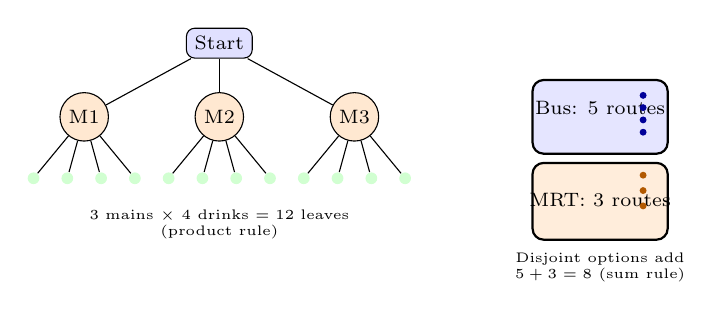
\begin{tikzpicture}[scale=0.78,every node/.style={font=\scriptsize},
  level 1/.style={sibling distance=2.2cm, level distance=1.2cm},
  level 2/.style={sibling distance=0.55cm, level distance=1.0cm}]
% left: lunch tree
\begin{scope}
\node[draw,rounded corners=3pt,fill=blue!12,inner sep=3pt] (r) at (0,1.6) {Start}
  child {node[draw,fill=orange!18,circle,inner sep=2pt] {M1}
    child {node[fill=green!18,circle,inner sep=1.5pt] {}}
    child {node[fill=green!18,circle,inner sep=1.5pt] {}}
    child {node[fill=green!18,circle,inner sep=1.5pt] {}}
    child {node[fill=green!18,circle,inner sep=1.5pt] {}}}
  child {node[draw,fill=orange!18,circle,inner sep=2pt] {M2}
    child {node[fill=green!18,circle,inner sep=1.5pt] {}}
    child {node[fill=green!18,circle,inner sep=1.5pt] {}}
    child {node[fill=green!18,circle,inner sep=1.5pt] {}}
    child {node[fill=green!18,circle,inner sep=1.5pt] {}}}
  child {node[draw,fill=orange!18,circle,inner sep=2pt] {M3}
    child {node[fill=green!18,circle,inner sep=1.5pt] {}}
    child {node[fill=green!18,circle,inner sep=1.5pt] {}}
    child {node[fill=green!18,circle,inner sep=1.5pt] {}}
    child {node[fill=green!18,circle,inner sep=1.5pt] {}}};
\node[font=\tiny,align=center] at (0,-1.35) {$3$ mains $\times$ $4$ drinks $=12$ leaves\\(product rule)};
\end{scope}
% right: sum rule
\begin{scope}[xshift=6.2cm]
\draw[thick,fill=blue!10,rounded corners=4pt] (-1.1,-0.2) rectangle (1.1,1.0);
\draw[thick,fill=orange!14,rounded corners=4pt] (-1.1,-1.6) rectangle (1.1,-0.35);
\node[font=\scriptsize] at (0,0.55) {Bus: 5 routes};
\node[font=\scriptsize] at (0,-0.95) {MRT: 3 routes};
\foreach \y in {0.15,0.35,0.55,0.75} \fill[blue!60!black] (0.7,\y) circle (1.6pt);
\foreach \y in {-0.55,-0.80,-1.05} \fill[orange!70!black] (0.7,\y) circle (1.6pt);
\node[font=\tiny,align=center] at (0,-2.05) {Disjoint options add\\$5+3=8$ (sum rule)};
\end{scope}
\end{tikzpicture}
\caption{Left: product rule as a branching tree. Right: sum rule as disjoint piles.}
\label{fig:product-sum}
\end{figure}

% ============================================================
\section{Product and Sum Rules}
\label{sec:product-sum}

\begin{theorem}[Product rule] If a task has $k$ sequential stages with $n_1,\dots,n_k$ choices respectively (choices at stage $i$ may depend on earlier choices but count is $n_i$), total outcomes $=n_1n_2\cdots n_k$.
\end{theorem}

\begin{theorem}[Sum rule] If sets $A_1,\dots,A_k$ are pairwise disjoint, $|A_1\cup\cdots\cup A_k|=|A_1|+\cdots+|A_k|$. For overlapping sets, see inclusion--exclusion (\S\ref{sec:inclusion}).
\end{theorem}

\begin{example}[Passwords] An $8$-character password over $62$ symbols: $62^8\approx2.18\times10^{14}$ possibilities. At $10^9$ guesses/sec, $\approx2.5$ days to brute-force. Product rule gives key-space size directly.
\end{example}

\subsection{Counting with Cases}
Often we partition by a property, count each case, then sum. This is sum rule in action. E.g., binary strings length $n$ with exactly $k$ ones: choose positions for the $k$ ones (see \S\ref{sec:combinations}).

% ============================================================
\section{Permutations}
\label{sec:permutations}
A \emph{permutation} is an ordered arrangement.

\begin{definition}[Permutation] The number of ordered arrangements of $k$ distinct items chosen from $n$ distinct items is
\[
P(n,k)=\frac{n!}{(n-k)!}=n(n-1)\cdots(n-k+1).
\]
When $k=n$, $P(n,n)=n!$.
\end{definition}

\emph{Why divide by $(n-k)!$?} Line up all $n!$ orders; the tail $n-k$ items beyond position $k$ are irrelevant---divide out their $(n-k)!$ orders.

\begin{example} Ranking top $3$ out of $10$ teams: $P(10,3)=10\cdot9\cdot8=720$. PIN codes of $4$ distinct digits from $10$: $P(10,4)=5040$.
\end{example}

\paragraph{Permutations with repetition.} If $n_1$ identical of type $1$, $n_2$ of type $2$, \dots, $n_r$ of type $r$ with $\sum n_i=n$,
\[
\frac{n!}{n_1!\,n_2!\cdots n_r!}.
\]
E.g., arrangements of \texttt{BANANA}: $6!/(3!\,2!\,1!)=60$.

% ============================================================
\section{Combinations}
\label{sec:combinations}

\begin{definition}[Combination] The number of ways to choose an unordered set of $k$ from $n$ distinct items is
\[
\binom{n}{k}=\frac{n!}{k!\,(n-k)!},\qquad 0\le k\le n.
\]
Read ``$n$ choose $k$''. By convention $\binom{n}{0}=1$.
\end{definition}

\begin{figure}[h]
\centering
\begin{tikzpicture}[scale=0.72,every node/.style={font=\scriptsize}]
% Pascal triangle colored
\foreach \r in {0,...,5} {
  \foreach \k in {0,...,\r} {
    \pgfmathsetmacro{\x}{(\k - \r/2)*1.15}
    \pgfmathsetmacro{\y}{-\r*0.62}
    \pgfmathtruncatemacro{\val}{1}
    % compute binomial coarsely for display
    \node[draw,circle,fill=blue!12,inner sep=1.8pt,minimum size=0.62cm] at (\x,\y) {
      \pgfmathparse{int(round(factorial(\r)/(factorial(\k)*factorial(\r-\k))))}\pgfmathresult
    };
  }
}
\node[font=\tiny,align=center] at (0,-4.0) {Pascal's triangle: $\binom{n}{k}=\binom{n-1}{k-1}+\binom{n-1}{k}$\\Each entry = sum of two above; colour groups by parity idea};
% stars and bars illustration
\begin{scope}[xshift=5.5cm,yshift=-0.3cm]
\node[font=\footnotesize\bfseries] at (1.5,0.8) {Stars and bars};
\foreach \i in {0,...,6} {\draw[thick] (\i*0.38,0) -- (\i*0.38,0.45);}
% stars as filled circles
\foreach \x in {0.19,0.57,1.14,1.52,1.90,2.28} \fill[orange!70!black] (\x,0.22) circle (2.2pt);
% bars as thick lines
\draw[ultra thick,red!70!black] (0.76, -0.05)--(0.76,0.5);
\draw[ultra thick,red!70!black] (1.90, -0.05)--(1.90,0.5);
\node[font=\tiny,align=center] at (1.3,-0.55) {$\star\star\mid\star\mid\star\star\star$ = $(2,1,3)$\\$x_1+x_2+x_3=6$};
\node[font=\tiny,align=center] at (1.3,-1.25) {$\binom{n+k-1}{k-1}$ ways};
\end{scope}
\end{tikzpicture}
\caption{Left: Pascal's triangle (binomial coefficients). Right: stars-and-bars encoding.}
\label{fig:pascal-stars}
\end{figure}

Key identities: $\binom{n}{k}=\binom{n}{n-k}$, $\binom{n}{k}=\binom{n-1}{k-1}+\binom{n-1}{k}$ (Pascal), $\sum_{k=0}^n\binom{n}{k}=2^n$, $\sum_k\binom{n}{k}^2=\binom{2n}{n}$.

\paragraph{Stars and bars.} Nonnegative integer solutions to $x_1+\dots+x_k=n$ correspond to placing $k-1$ bars among $n+k-1$ slots:
\[
\binom{n+k-1}{k-1}.
\]
For positive solutions ($x_i\ge1$), shift $y_i=x_i-1$: $\binom{n-1}{k-1}$. Example: distributing $10$ identical tasks to $4$ servers: $\binom{13}{3}=286$ ways.

% ============================================================
\section{Binomial Theorem and Inclusion--Exclusion}
\label{sec:inclusion}
\begin{theorem}[Binomial theorem] For any $x,y$ and $n\ge0$,
\[
(x+y)^n=\sum_{k=0}^n\binom{n}{k}x^k y^{n-k}.
\]
Setting $x=y=1$ gives $\sum_k\binom{n}{k}=2^n$. Setting $x=1,y=-1$ gives alternating sum $0$.
\end{theorem}

\begin{example}[Committee with a chair] Choose a $k$-person committee from $n$ and a chair among them: $k\binom{n}{k}=n\binom{n-1}{k-1}$ ways (pick chair first vs.\ committee first). Summing over $k$ gives $\sum_k k\binom{n}{k}=n2^{n-1}$, a useful identity for expected value of $\mathrm{Bin}(n,1/2)$.
\end{example}

\begin{theorem}[Inclusion--exclusion, two and three sets]
\[
|A\cup B|=|A|+|B|-|A\cap B|,\quad |A\cup B\cup C|=\sum|A_i|-\sum|A_i\cap A_j|+|A\cap B\cap C|.
\]
In general, add singles, subtract pairs, add triples, \dots.
\end{theorem}

\begin{example}[Derangements via inclusion--exclusion] Counting surjections or derangements uses the full alternating sum; e.g., onto functions $[n]\to[k]$ count $=k!\,S(n,k)=\sum_{j=0}^k(-1)^j\binom{k}{j}(k-j)^n$.
\end{example}

% ============================================================
\section{The Pigeonhole Principle}
\label{sec:pigeonhole}
\begin{theorem}[Pigeonhole principle] If $n$ pigeons go into $k$ holes with $n>k$, some hole has $\ge2$ pigeons. Generalised: some hole has $\ge\lceil n/k\rceil$ pigeons.
\end{theorem}

This proves \emph{existence} without construction. In computing: with $2^n+1$ files each $n$ bits, two share the same $n$-bit hash (collision). With $367$ people, two share a birthday (including Feb~29). In any $6$ people, $3$ mutually know each other or $3$ mutually strangers (Ramsey $R(3,3)=6$).

\begin{figure}[h]
\centering
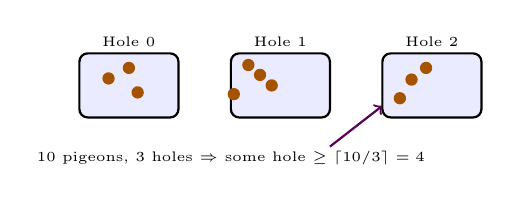
\begin{tikzpicture}[scale=0.74,every node/.style={font=\scriptsize}]
\foreach \i in {0,1,2} {
  \draw[thick,fill=blue!8,rounded corners=3pt] (\i*2.6-2.6,-0.55) rectangle (\i*2.6-2.6+1.7,0.55);
  \node[font=\tiny] at (\i*2.6-1.75,0.75) {Hole \i};
}
% pigeons as colored circles
\foreach \x/\y in {-2.1/0.12,-1.6/-0.12,-1.75/0.30, 0.5/0.18,0.05/-0.15,0.7/0.0,0.3/0.35, 3.1/0.1,2.9/-0.22,3.35/0.30} \fill[orange!65!black] (\x,\y) circle (3pt);
\node[font=\tiny,align=center] at (0,-1.25) {$10$ pigeons, $3$ holes $\Rightarrow$ some hole $\ge\lceil10/3\rceil=4$};
\draw[->,thick,violet!70!black] (1.7,-1.05)--(2.6,-0.35);
\end{tikzpicture}
\caption{Pigeonhole principle: more pigeons than holes forces a crowded hole.}
\label{fig:pigeonhole}
\end{figure}

% ============================================================
\section{Counting in Code}
\label{sec:code-counting}
Counting formulas become code when enumerating. Python's \texttt{math.comb} and \texttt{math.perm} implement $\binom{n}{k}$ and $P(n,k)$ exactly with big integers.

\begin{lstlisting}[language=Python]
import math
# key-space and combinations in computing
print(math.perm(10, 3))          # 720 rankings
print(math.comb(50, 5))          # 2_118_760 feature subsets
print(math.comb(10+4-1, 4-1))   # 286 task distributions (stars/bars)
# brute-force estimate: 62^8 passwords
print(62**8, " ~ 2.2e14")
# verify binomial identity sum_k C(n,k) == 2^n
n = 20
assert sum(math.comb(n, k) for k in range(n+1)) == 2**n
\end{lstlisting}

% ============================================================
\section{Chapter Notes}
Dirichlet stated the pigeonhole (Schubfach) principle in 1834. Stars-and-bars is folk combinatorics; see Feller Vol.~1. Binomial coefficients appear in Knuth TAOCP Vol.~1 and CLRS App.~C. For large $n$, Stirling $n!\sim\sqrt{2\pi n}(n/e)^n$ estimates key spaces without overflow.

% ============================================================
\section{Exercises}
\label{sec:ch01-exercises}
\begin{enumerate}[label=E1.\arabic*, leftmargin=*, itemsep=0.8em]
\item \textbf{Product vs.\ sum.} A system offers $4$ operating systems, each with $6$ desktop environments, plus $3$ standalone window managers usable with any OS. How many distinct software stacks? Identify where product vs.\ sum applies and compute the total.
\item \textbf{Permutations with repetition.} How many distinct strings can be formed from \texttt{MISSISSIPPI}? Generalise to a multiset with counts $n_1,\dots,n_r$ and verify your formula gives $60$ for \texttt{BANANA}.
\item \textbf{Stars and bars.} (a) How many nonnegative integer solutions to $x_1+x_2+x_3+x_4=12$? (b) How many \emph{positive} solutions? (c) A load balancer distributes $12$ identical requests to $4$ servers, each must get $\ge1$. Count assignments.
\item \textbf{Inclusion--exclusion.} Among $100$ students, $60$ know Python, $50$ know Java, $30$ know both. How many know neither? Extend: with a third language ($40$ know C, pairwise overlaps $20,15,18$, triple $8$), how many know at least one?
\item \textbf{Pigeonhole in hashing.} A hash table has $1000$ buckets and stores $1001$ distinct keys with a deterministic hash function. Prove a collision must occur. If $5000$ keys are stored, give a lower bound on the maximum bucket occupancy.
\end{enumerate}
% End of Chapter 1
